\paragraph{Probes.}
We index time by the agent's column relative to the passage and bin it into an
evidence phase, a corridor phase and the passage. On states $\mathbf{h}_t$
collected from held-out maps, split by map into $801$ maps for fitting and
$399$ for testing, we train a logistic-regression probe and a one-hidden-layer
MLP probe to predict the three-way category at each bin, against a
shuffled-label null. The gap between the two probes measures how non-linear
the code is.

\paragraph{The single direction.}
Let $\mu_{\mathrm r}$ and $\mu_{\mathrm l}$ be the means of $\mathbf{h}_t$ over
the eight columns immediately before the passage on rocky and lakes training
maps; $\mathbf{v}=(\mu_{\mathrm r}-\mu_{\mathrm l})/\lVert\mu_{\mathrm r}-\mu_{\mathrm l}\rVert$.
An episode's belief $\hat b$ is $b_t=\mathbf{h}_t^{\top}\mathbf{v}$ averaged
over the same eight columns before the first passage crossing; the class means
of $\hat b$ are the category poles $b^{\star}_{\text{rocky}}$ and $b^{\star}_{\text{lakes}}$
and their midpoint $m$ the decision boundary, and an
episode has \emph{crossed} when $\hat b$ lies on the other side of $m$ from its
unsteered value. To price the reduction from $128$ dimensions to one we fit a
logistic regression on $\hat b$ alone and one on the full state under
five-fold cross-validation over training maps, refitting $\mathbf{v}$ inside
each fold so the whole pipeline is scored. Balanced maps are never used to fit
$\mathbf{v}$.

\paragraph{Causal test.}
We write to the coordinate and leave every other direction untouched,
\begin{equation}
\mathbf{h}' \;=\; \mathbf{h} + \big(b_{\lambda} - \mathbf{h}^{\top}\mathbf{v}\big)\,\mathbf{v},
\qquad
b_{\lambda} \;=\; (1-\lambda)\,b^{\star}_{\text{own}} + \lambda\,b^{\star}_{\text{other}},
\label{eq:set}
\end{equation}
where $b^{\star}_{\text{own}}$ is the pole of the map's true category,
$b^{\star}_{\text{other}}$ that of the other labelled category, and $\lambda$
the dose: $\lambda=0$ writes the agent's own category, a null write that
should change nothing, and $\lambda=1$ writes the opposite category. The write is applied once at corridor entry
(transient) or at every step from entry (sustained). The outcome is the flag
taken; on balanced maps we set $b_{\lambda}$ to each category's pole and report the top-flag rate.
The control writes the same displacement $\lVert\mathbf{h}'-\mathbf{h}\rVert$
along random unit directions on the same maps with the same timing.

\paragraph{Position bins and the geometry of the belief.}
All per-bin analyses use the eight bins of Figure~\ref{fig:bins}: five over the
evidence terrain, two over the memory corridor, and one at the passage.
Figure~\ref{fig:pca} projects the per-map bin means of lakes and rocky maps on
the first two principal components of those states, with the per-bin
difference-of-means direction drawn as a segment between the two class means.
Figure~\ref{fig:pca_balanced} shows each category separately in that plane with its per-bin mean.

\begin{figure}[t]
\centering
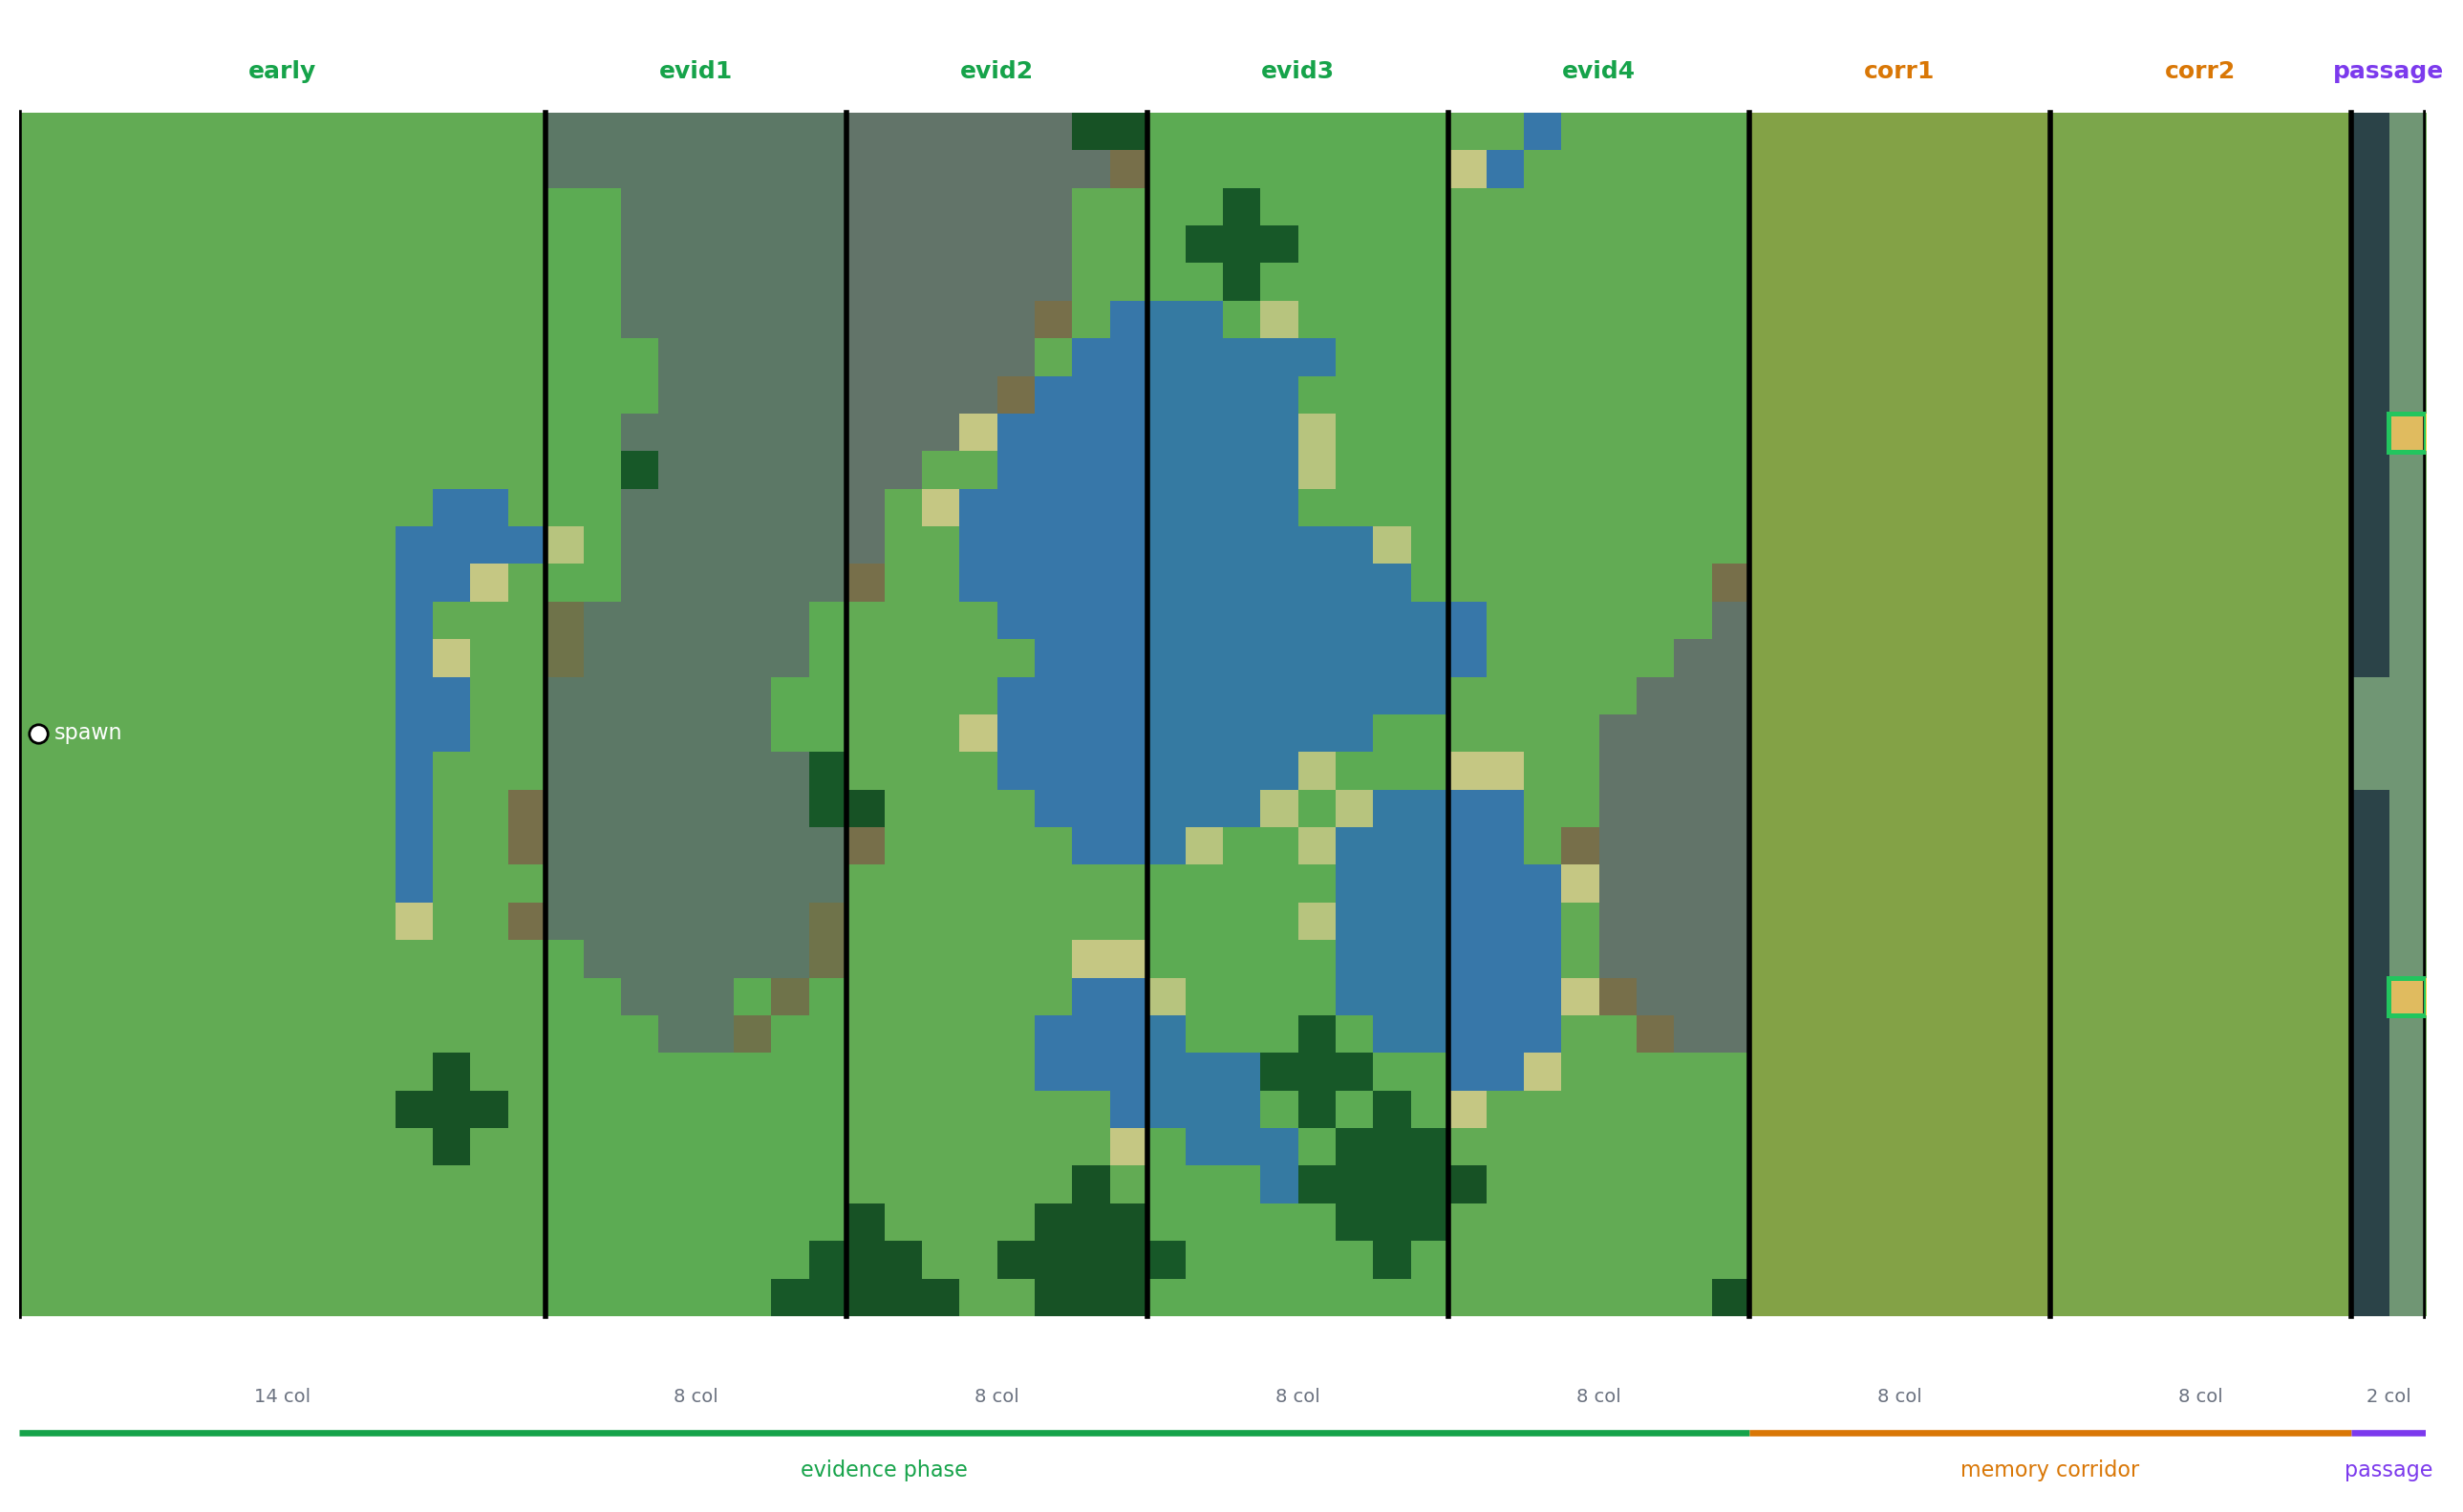
\includegraphics[width=\linewidth]{figures/fig_bins.png}
\caption{\textbf{The eight position bins}, drawn on a held-out balanced map.
Episodes are aligned by the agent's column relative to the passage rather than
by time, so agents of different speeds are compared at the same place. Five
bins cover the evidence terrain, two the memory corridor, and one the passage.}
\label{fig:bins}
\end{figure}

\begin{figure}[t]
\centering
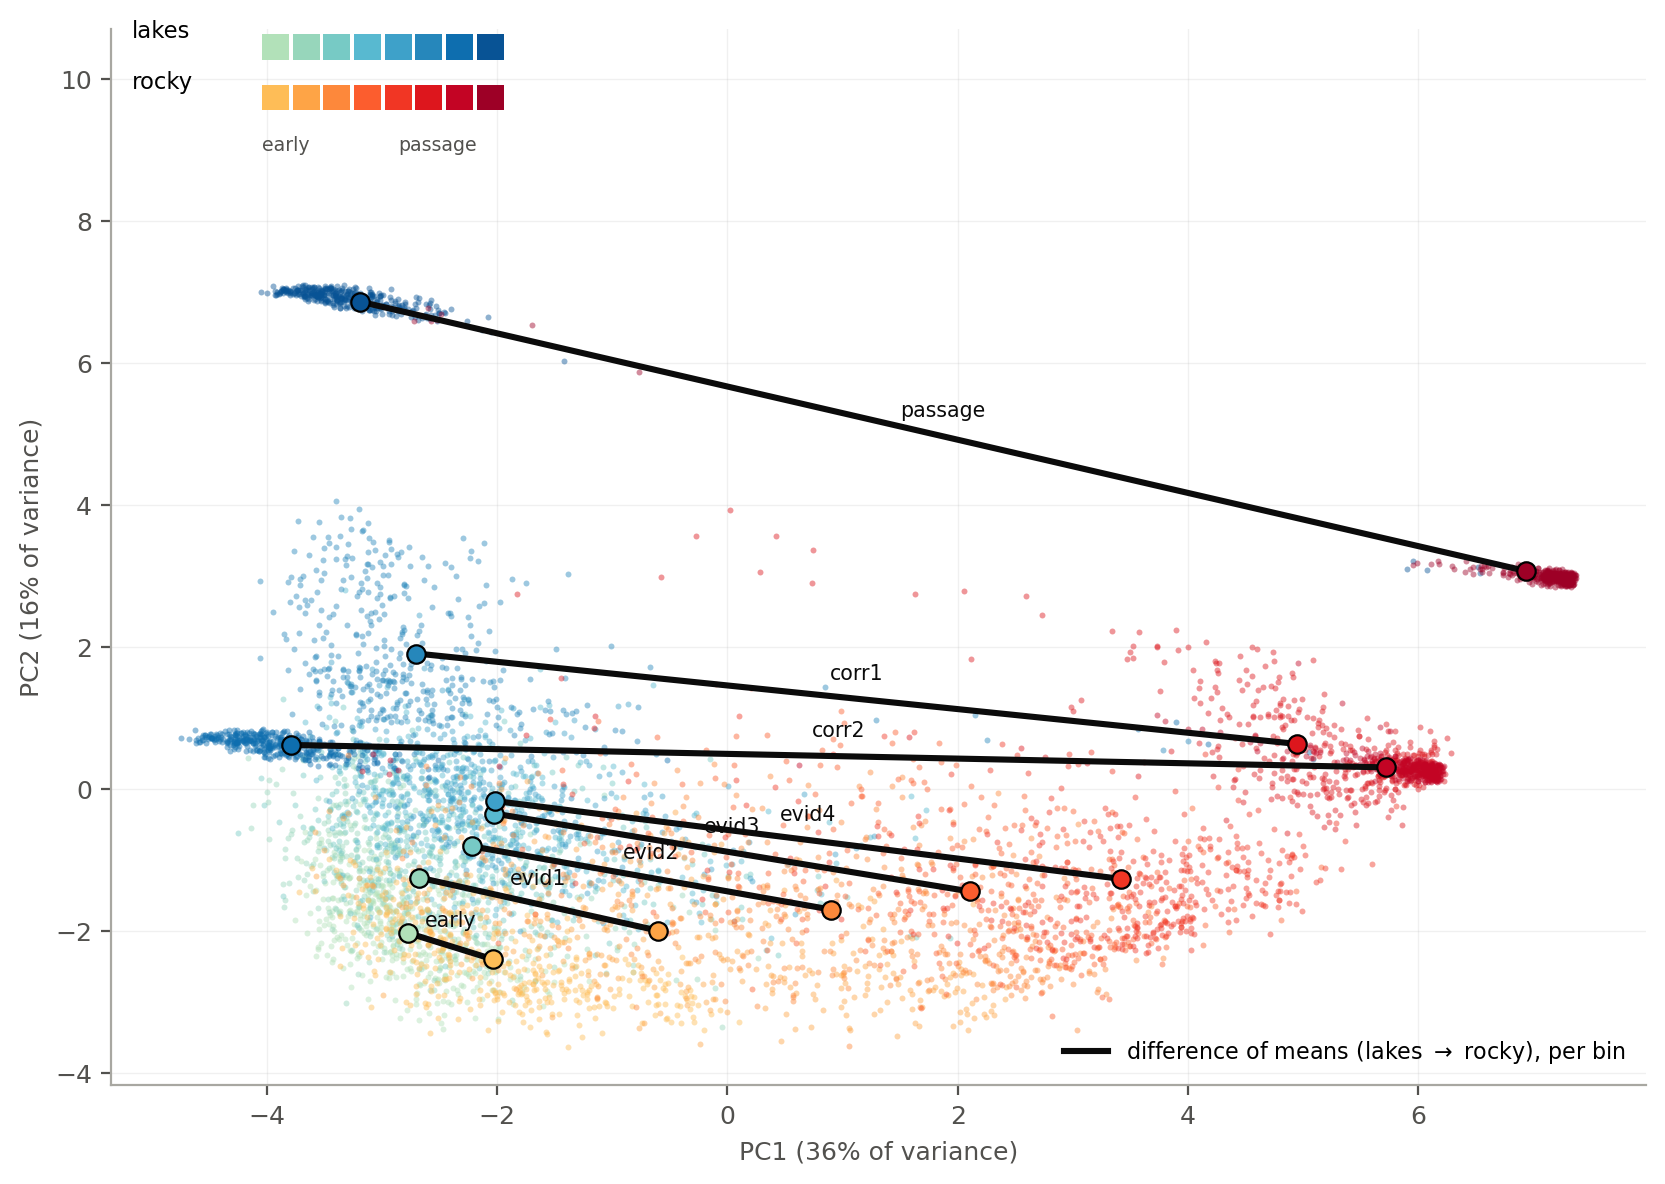
\includegraphics[width=0.9\linewidth]{figures/fig_pca_lakes_rocky.png}
\caption{\textbf{Lakes and rocky states in the first two principal
components.} One point per map and bin, hue for the category and lightness for
the bin; segments join the lakes and rocky class means of each bin, i.e.\ the
per-bin single direction. PC1 seems to encode the rocky belief: rocky states
move steadily to the right as evidence accumulates and pin at the far right by
the passage. PC2 seems to encode the lakes belief: lakes states stay left and
rise sharply in the corridor and at the passage. The two categories therefore
separate along different axes late in the episode, and the difference-of-means
direction rotates accordingly.}
\label{fig:pca}
\end{figure}

\begin{figure}[t]
\centering
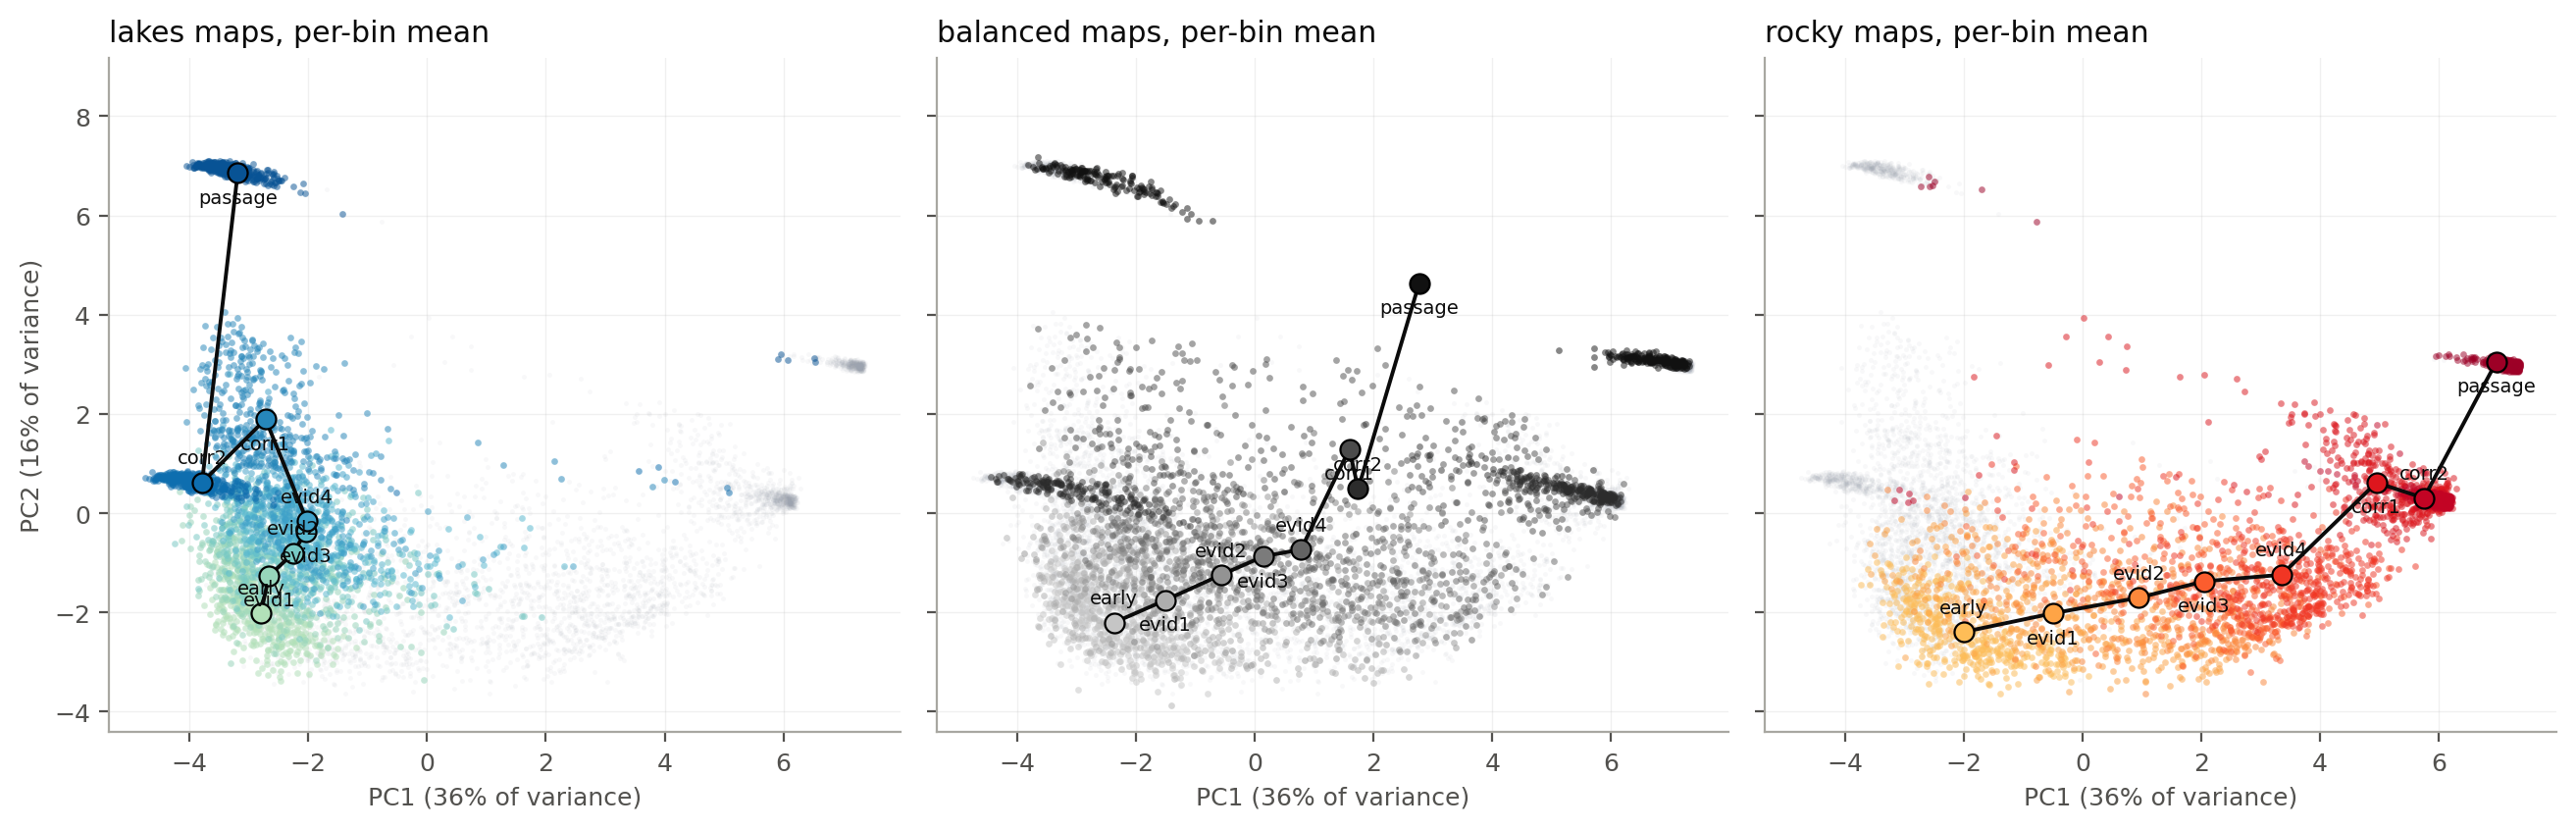
\includegraphics[width=\linewidth]{figures/fig_pca_categories.png}
\caption{\textbf{Each category in the same plane, with its per-bin mean.} The
plane is the one of Figure~\ref{fig:pca}, fitted on lakes and rocky states;
the full lakes-and-rocky cloud is drawn faintly in every panel for reference,
points are shaded by bin and the black path joins the per-bin means. Lakes
maps stay left and rise sharply in the corridor and at the passage. Balanced
maps, never used to fit the plane, travel up the middle early on, but by the
passage their points lie on the lakes arm or the rocky arm rather than in
between, so the mean sits between two occupied poles. Rocky maps move steadily
right and settle at the far right. A balanced map is not held as ``undecided''; the
agent commits to one category and walks to its flag.}
\label{fig:pca_balanced}
\end{figure}
